% !TEX root = 02.tex

\section{Analysis Passes}


\begin{frame}{Checking Input Properties}
Analyses basically allow to:
\begin{itemize}
\item \alert{derive} information and properties of the input
\item \alert{verify} properties of input
\end{itemize}

\vfill
Keeping analyzed information updated is expensive:
\begin{itemize}
\item tuned algorithms update information when an optimization
      invalidates it
\item incrementally updating analyses are cheaper than recomputing them
\end{itemize}

\vfill
As an \alert{optimization}, many LLVM analysis supports incremental updates.
\end{frame}


\begin{frame}{Useful Analyses}
\begin{center}
We will see the following passes:\\
\bigskip
\begin{tabular}{ccc}
\toprule

\multicolumn{1}{c}{\textbf{Pass}}        &
\multicolumn{1}{c}{\textbf{Switch}}      &
\multicolumn{1}{c}{\textbf{Transitive}} \\

\midrule

Control flow graph  &
---       &
No                 \\

Dominator tree    &
\texttt{domtree}  &
No               \\

Post-dominator tree   &
\texttt{postdomtree}  &
No                   \\

Loop information  &
\texttt{loops}    &
Yes              \\

Scalar evolution           &
\texttt{scalar-evolution}  &
Yes                       \\

Alias analysis    &
\texttt{special}  &
Yes              \\

Memory dependence  &
\texttt{memdep}    &
Yes               \\

\bottomrule
\end{tabular}
\end{center}
\end{frame}


\begin{frame}{Requesting an Analysis}
\begin{center}
Your pass needs to tell the pass manager which analyses it needs!

\vfill
Transitive analyses:\\
\cppinline{llvm::AnalysisUsage::addRequiredTransitive<T>()}\\
\medskip
Non-transitive analyses: \\
\cppinline{llvm::AnalysisUsage::addRequired<T>()}\\

\vfill
For \alert{chained analyses}\footnote{Analyses that use the result of another analysis}, the \texttt{addRequiredTransitive} method
should be used instead of the \texttt{addRequired} method.\\
\medskip
{\small
This informs the PassManager that the transitively required pass
should be alive as long as the requiring pass is.}
\end{center}
\end{frame}


\subsection{Control Flow Graph}


\begin{frame}{Control Flow Graph}
The Control Flow Graph is implicitly maintained by LLVM:

\begin{itemize}
\item no specific pass to build it
\end{itemize}

\vfill
Recap:

\begin{itemize}
\item CFG for a function is a graph of basic blocks
\item a basic block is a list of instructions
\end{itemize}

\vfill
Functions and basic blocks act like containers:

\begin{itemize}
\item STL-like accessors: \cppinline{front()}, \cppinline{back()},
      \cppinline{size()}, \ldots
\item STL-like iterators: \cppinline{begin()}, \cppinline{end()}
	\begin{itemize}
	\item Warning for BBs: order of iteration $\neq$ order of execution!
	\end{itemize}
\end{itemize}

\vfill
Each contained element is aware of its container:

\begin{itemize}
\item \cppinline{getParent()}
\end{itemize}
\end{frame}


\begin{frame}{Control Flow Graph}{Walking}
Every CFG has an \alert{entry} basic block:

\begin{itemize}
\item the \alert{first} executed basic block
\item it is the \alert{root/source} of the graph
\item get it with \cppinline{llvm::Function::getEntryBlock()}
\end{itemize}

\vfill
At the end of a basic blocks there's always a \alert{terminator} instruction:
\begin{itemize}
\item \llvminline{ret}, \llvminline{br}, \llvminline{switch}, \llvminline{unreachable}, \ldots
\end{itemize}

\vfill
More than one \alert{exit} block can be present in a function:

\begin{itemize}
\item they are the \alert{leaves/sinks} of the graph
\item their terminator instructions are always \llvminline{ret}s
\begin{enumerate}
\item \cppinline{llvm::BasicBlock::getTerminator()}
\item check the opcode of the terminator
\end{enumerate}
\end{itemize}
\end{frame}


\begin{frame}{Side Note}{Casting Framework}
For performance reasons, a custom casting framework is used:

\begin{itemize}
\item you cannot use \cppinline{static\_cast} and \cppinline{dynamic\_cast} with
      types/classes provided by LLVM
\end{itemize}

\begin{block}{LLVM Casting Functions}
\centering
\medskip
\begin{tabular}{rl}

Static cast of \cppinline{Y*} to \cppinline{X}  &
\cppinline{X *llvm::cast<X>(Y *)}                \\

Dynamic cast of \cppinline{Y*} to \cppinline{X}  &
\cppinline{X *llvm::dyn\_cast<X>(Y *)}            \\

Is \cppinline{Y*} an instance of \cppinline{X}?  &
\cppinline{bool llvm::isa<X>(Y *)} \\

\end{tabular}
\smallskip
\end{block}

Example:

\begin{itemize}
\item is \cppinline{BB} a sink?\\
      \cppinline{llvm::isa<llvm::ReturnInst>(BB.getTerminator())}
\end{itemize}
\end{frame}


\begin{frame}{Control Flow Graph}{Basic Blocks}
Every basic block \cppinline{BB} has one or more\footnote{see include/llvm/IR/CFG.h}:

\begin{description}[predecessors]
\item[predecessors] from \cppinline{pred\_begin(BB)} to
      \cppinline{pred\_end(BB)}
\item[successors] from \cppinline{succ\_begin(BB)} to
      \cppinline{succ\_end(BB)}
\end{description}

\vfill
Other convenience methods available in \cppinline{llvm::BasicBlock}:

\begin{itemize}
\item useful getters
\begin{itemize}
\item \cppinline{BasicBlock *getUniquePredecessor()}
\item \ldots
\end{itemize}
\item moving a basic block
\begin{itemize}
\item      \cppinline{moveBefore(llvm::BasicBlock *)}
\item      \cppinline{moveAfter(llvm::BasicBlock *)}
\end{itemize}
\item split a basic block:
\begin{itemize}
\item      \cppinline{splitBasicBlock(llvm::BasicBlock::iterator)}
\end{itemize}
\item \ldots
\end{itemize}
\end{frame}


\begin{frame}{Control Flow Graph}{Instructions}
The \cppinline{llvm::Instruction} class defines common operations: \\
\medskip
\begin{itemize}
\item getting an operand
\begin{itemize}
\item \cppinline{getOperand(unsigned)}
\end{itemize}
\end{itemize}
\vfill
Subclasses provide specialized accessors: \\
\medskip
\begin{itemize}
\item the \llvminline{load} instruction takes as operand the pointer to the memory to be loaded:
\begin{itemize}
\item      \cppinline{llvm::LoadInst::getPointerOperand()}
\end{itemize}
\end{itemize}
\end{frame}


\begin{frame}{Instructions}{Creating New Instructions}
Instructions are created using:

\begin{itemize}
\item constructors
\begin{itemize}
\item \cppinline{llvm::LoadInst::LoadInst(...)}
\end{itemize}
\item factory methods
\begin{itemize}
\item \cppinline{llvm::GetElementPtrInst::Create(...)}
\end{itemize}
\item the helper class \cppinline{llvm::IRBuilder}
\begin{itemize}
\item \cppinline{llvm::IRBuilder<> builder(insPoint);}\\
\cppinline{builder.CreateAdd(...);}
\end{itemize}
\end{itemize}
\vfill
\alert{Interface is not homogeneous!}\\
Some instructions support all methods, others support only one.
\end{frame}


\begin{frame}{Instructions}{Inserting New Instructions}


\vfill
Instructions can be inserted:
\vfill
\begin{itemize}
\item automatically by \cppinline{IRBuilder}
\begin{itemize}
\item insertion point is given at \cppinline{IRBuilder} instantiation
\end{itemize}
\bigskip
\item manually by appending to a basic block
\item manually by inserting after/before another instruction
\end{itemize}
\vfill
\end{frame}


\begin{frame}{From Control Flow to Data Flow}{Definitions and Uses}
In LLVM, the data flow generated by the various instructions is represented by a simple hierarchy:

\begin{description}[valueMMM]
\item[value] something that can be used: \cppinline{llvm::Value}
\item[user] something that can use: \cppinline{llvm::User}
\item[use] the link between the \alert{value} and the \alert{user}: \cppinline{llvm::Use}
\end{description}
\medskip
A value is a \alert{definition}:

\begin{itemize}
\item Visiting where a definition is used:
\begin{itemize}
\item \cppinline{llvm::Value::use\_begin()}, \cppinline{llvm::Value::use\_end()}
\end{itemize}
\end{itemize}
\medskip
An user accesses \alert{definitions}:

\begin{itemize}
\item Visiting the definitions that are used:
\begin{itemize}
\item \cppinline{llvm::User::op\_begin()}, \cppinline{llvm::User::op\_end()}
\end{itemize}
\end{itemize}
\medskip

\end{frame}


\begin{frame}{From Control Flow to Data Flow}{Instructions are Values}
\vfill
\begin{itemize}
\item \cppinline{llvm::Value} inherits from \cppinline{llvm::User}
\item \cppinline{llvm::Instruction} inherits from \cppinline{llvm::Value}
\begin{itemize}
\normalsize
\item[$\Rightarrow$] The value produced by the instruction is\\the \alert{instruction itself}!
\end{itemize}
\end{itemize}

\begin{block}{Example}
\begin{center}
\llvminline{\%6 = load i32, i32* \%1, align 4}\\
\medskip
The \llvminline{load} is described by an instance of \cppinline{llvm::Instruction}. \\
That instance also represents the \llvminline{\%6} variable. \\
\end{center}
\end{block}

\begin{center}
Not all instances of \cppinline{llvm::Value} are also \cppinline{llvm::Instruction}s!\\
\smallskip
{\small i.e. function arguments}

\end{center}
\vfill
\end{frame}


\begin{frame}{From Control Flow to Data Flow}{Value Typing}
Every \cppinline{llvm::Value} is typed:

\begin{itemize}
\item use \cppinline{llvm::Value::getType()} to get the type
\end{itemize}

\vfill
Since every instruction is a value:

\begin{itemize}
\item instructions are typed
\end{itemize}

\vfill
\begin{block}{Example}
\begin{center}
\llvminline{\%6 = load i32, i32* \%1, align 4}\\
\medskip
The type of the \llvminline{\%6} variable is the type of the return value of the \llvminline{load} instruction, \llvminline{i32}\\
\end{center}
\end{block}
\end{frame}


%\begin{frame}{From Control Flow to Data Flow}{Instructions are like functions}
%\vfill
%\vfill
%\begin{columns}[t]
%\column{.45\textwidth}
%Functions:
%
%\begin{itemize}
%\item used by call sites
%\item uses formal parameters
%\end{itemize}
%
%\column{.45\textwidth}
%Instructions:
%
%\begin{itemize}
%\item define an SSA value
%\item uses operands
%\end{itemize}
%\end{columns}
%
%\vfill
%\vfill
%\end{frame}


\subsection{Dominance Trees}


\begin{frame}{Dominance Trees}
Dominance trees answer to control-related queries:\\

\vfill
\begin{columns}[onlytextwidth]
\column{.475\textwidth}
\begin{centering}
is \texttt{A} executed \alert{before} \texttt{B}?\\
$\Downarrow$\\
\cppinline{llvm::DominatorTree}\\
\end{centering}

\column{.525\textwidth}
\begin{centering}
is \texttt{A} executed \alert{after} \texttt{B}?\\
$\Downarrow$\\
\cppinline{llvm::PostDominatorTree}\\
\end{centering}
\end{columns}

\vfill
The interfaces of these two trees is mostly the same:

\begin{itemize}
\item \cppinline{bool dominates(A, B)}
\item \cppinline{bool properlyDominates(A, B)}
\end{itemize}

\cppinline{A} and \cppinline{B} are either
\cppinline{llvm::BasicBlock}s or
\cppinline{llvm::Instruction}s

\vfill
By using \texttt{opt}, it is possible to show the trees:

\begin{itemize}
\item \aligntext{\texttt{-view-postdom},}{\texttt{-view-dom},} \texttt{-dot-dom}
\item \aligntext{\texttt{-view-postdom},}{\texttt{-view-postdom},} \texttt{-dot-postdom}
\end{itemize}
\end{frame}


\subsection{Loop Information}


\begin{frame}{Loop Information}
Loop information is represented using two classes:

\begin{description}[\texttt{llvm::LoopInfo}]
\item[\texttt{llvm::LoopInfo}]
			The result of \cppinline{llvm::LoopAnalysis},\\
			performed on a given function.
\item[\texttt{llvm::Loop}]
			Represents a single loop in a function.\\
			Contained inside a \texttt{llvm::LoopInfo}.
\end{description}

\vfill
Using \cppinline{llvm::LoopInfo} it is possible:

\begin{itemize}
\item navigate through top-level loops:
\begin{itemize}
\item \cppinline{llvm::LoopInfo::begin()}
\item \cppinline{llvm::LoopInfo::end()}
\end{itemize}
\item get the loop for a given basic block:
\begin{itemize}
\item \cppinline{llvm::LoopInfo::operator[](llvm::BasicBlock *)}
\end{itemize}
\end{itemize}
\end{frame}


\begin{frame}{Loop Information}{Nesting Tree}
Loops are represented as a \alert{tree}:\\
\begin{columns}
\column{.6\textwidth}
\begin{block}{Source\vphantom{Loop Nest}}
\cinput[\tt\fontsize{7.5pt}{7.5pt}\selectfont]{snippet/loop-nest.c}
\end{block}
\column{.3\textwidth}
\begin{block}{Loop Hierarchy}
\centering

% loop-nest.tex: a simple loop nest.

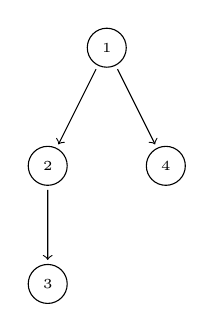
\begin{tikzpicture}
[
  every node/.style={
    font=\tiny
  },
  loop/.style={
    circle,
    draw
  },
  tip/.style={
    shorten <=.5mm,
    shorten >=.5mm,
    ->,
    draw
  },
  level 1/.style={
    edge from parent/.style=tip
  },
]

\node [loop] {$1$}
  child { node [loop] {$2$}
    child { node [loop] {$3$}}
  }
  child { node [loop] {$4$}};
\end{tikzpicture}

\end{block}
\end{columns}
\vfill
\begin{description}[children loops]
\item[children loops] \cppinline{llvm::Loop::begin()},
      \cppinline{end()}
\item[parent loop] \cppinline{llvm::Loop::getParentLoop()}
\end{description}
\end{frame}


\begin{frame}{Loop Information}{Query Loops}
Accessors for important nodes:

\begin{description}
\item[pre-header] \cppinline{llvm::Loop::getLoopPreheader()}
\item[header] \cppinline{llvm::Loop::getHeader()}
\item[latch] \cppinline{llvm::Loop::getLoopLatch()}
\item[exiting] \cppinline{llvm::Loop::getExitingBlock()}, \\
               \cppinline{llvm::Loop::getExitingBlocks(...)}
\item[exit] \cppinline{llvm::Loop::getExitBlock()} \\
            \cppinline{llvm::Loop::getExitBlocks(...)}
\end{description}

\vfill
The list of all BBs in the loop is accessible via:

\begin{description}
\item[iterators] \cppinline{llvm::Loop::block\_begin()}, \\
                 \cppinline{llvm::Loop::block\_end()}
\item[vector]
      \texttt{\addfontfeature{LetterSpace=-5}std::vector<BasicBlock *> \&Loop::getBlocks()}
\end{description}
\end{frame}


\subsection{Scalar Evolution}


\begin{frame}{Scalar Evolution}
The \alert{SC}alar \alert{EV}olution pass analyzes scalar
expressions inside loops.

\begin{itemize}
\item all expressions are categorized and represented uniformly
\item is capable of handling \alert{general induction variables}
\item also useful outside of loops
\item \texttt{opt} flags: \texttt{-analyze -scalar-evolution}
\end{itemize}

\vfill
\begin{columns}[onlytextwidth]
\column{.67\textwidth}
\begin{block}{Example}
\llvminput[\tt\scriptsize]{snippet/basic-scev.ll}
\end{block}

\column{.30\textwidth}
SCEV for \llvminline{\%i.0}:

\begin{itemize}
\item initial value $0$
\item incremented \\by $1$ at each iteration
\item final value $10$
\end{itemize}
\end{columns}
\end{frame}


\begin{frame}{Scalar Evolution}{Example}
\begin{columns}
\column{.55\textwidth}
\begin{block}{Source}
\cinput[\tt\small]{snippet/nested-scev.c}
\end{block}

\column{.35\textwidth}
SCEV \llvminline{\{A,B,C\}<\%D>}:

\begin{itemize}
\item \llvminline{A} starting value
\item \llvminline{B} operator
\item \llvminline{C} stride
\item \llvminline{D} loop head BB
\end{itemize}

\llvminline{\{0,+,1\}=0+1+1+1+}\ldots

\end{columns}

\vfill
\begin{block}{Induction Variables}
\centering
\llvminput[\tt\small]{snippet/nested-scev-induction.ll}
\end{block}
\end{frame}


\begin{frame}{Scalar Evolution}{More than Induction Variables}
The scalar evolution framework manages \alert{any scalar expression}:

\begin{block}{Pointer SCEVs in two nested loops}
\centering
\llvminput[\tt\footnotesize]{snippet/nested-scev-pointer.ll}
\end{block}

\vfill
SCEV is an analysis used by many common optimizations
\begin{itemize}
\small
\item induction variable substitution
\item strength reduction
\item vectorization
\item \ldots
\end{itemize}
\end{frame}


\begin{frame}{Scalar Evolution}{SCEVs Design}
SCEVs are modeled by the \cppinline{llvm::SCEV} class:

\begin{itemize}
\item a subclass for each kind of SCEV: e.g. \cppinline{llvm::SCEVAddExpr}
\item instantiation disabled
\end{itemize}

\vfill
A SCEV actually is a tree of SCEVs:

\begin{itemize}
\item \llvminline{\{(80 + \%bar),+,80\}} =
\begin{itemize}
\item			\llvminline{\{\%1,+,80\}}
\item     \llvminline{\%1 = 80 + \%bar}
\end{itemize}
\end{itemize}

Tree leaves:

\begin{description}
\item[constant] \cppinline{llvm::SCEVConstant}: e.g. \llvminline{80}
\item[unknown\footnote{Not further splittable}] \cppinline{llvm::SCEVUnknown}:
                                                 e.g. \llvminline{\%bar}
\end{description}

\vfill
SCEV tree explorable through the visitor pattern:

\begin{itemize}
\item \cppinline{llvm::SCEVVisitor}
\end{itemize}
\end{frame}


\begin{frame}{Scalar Evolution}{Analysis Interface}
\centering
The \cppinline{llvm::ScalarEvolutionAnalysis} pass computes all the
SCEVs for a given \cppinline{llvm::Function}.
\vfill
\centering
The \cppinline{llvm::ScalarEvolution} instance produced by the pass
provides the following services:
\vfill
\begin{itemize}
\item get the SCEV representing a value:
\begin{itemize}
\item      \cppinline{getSCEV(llvm::Value *)}
\end{itemize}
\vfill
\item get important SCEVs from other structures or SCEVs:
\begin{itemize}
\item      \cppinline{getBackedgeTakenCount(llvm::Loop *)}
\item      \cppinline{getPointerBase(llvm::SCEV *)}
\item      \ldots
\end{itemize}
\vfill
\item create new SCEVs explicitly:
\begin{itemize}
\item \cppinline{getConstant(llvm::ConstantInt *)}
\item \cppinline{getAddExpr(llvm::SCEV *, llvm::SCEV *)}
\item \ldots
\end{itemize}
\end{itemize}
\end{frame}


\subsection{Alias Analysis}


\begin{frame}{Alias Analysis}
Let $X$ be an instruction accessing a memory location:

\begin{itemize}
\item is there another instruction accessing the same location?
\end{itemize}

\vfill
Alias analysis tries to answer the question:

\begin{description}
\item[application] optimization of memory operations
\item[problem] often fails
\end{description}

\vfill
Different algorithms are available for alias analysis:

\begin{itemize}
\item common interface: \cppinline{llvm::AliasAnalysis}
\item base implementation: basic alias analysis (\texttt{basicaa})
\end{itemize}

\begin{block}{Requiring Alias Analysis}
\centering
\cppinput{snippet/requiring-alias-analysis.cpp}
\end{block}
\end{frame}


\begin{frame}{Alias Analysis}{Memory Representation}
\begin{columns}
\column{.45\textwidth}
\begin{block}{Source}
\centering
\llvminput[\tt\footnotesize]{snippet/memory-locations.ll}
\end{block}

\centering
\bigskip
Basic building block:\\\texttt{llvm::AliasAnalysis::}\\\texttt{Location}

\begin{itemize}
\item address: e.g. \llvminline{\%a}
\item size: e.g. 2 bytes
\end{itemize}

\column{.45\textwidth}
\begin{block}{Distinct Locations}
\centering

% alias-analysis-distinct.tex: different locations.

\begin{tikzpicture}
[
  every node/.style={
    font=\tiny
  },
  location/.style={
    rectangle split,
    rectangle split parts=2,
    rotate=90,
    draw
  },
  location-a/.style={
    location,
    rectangle split part fill={
      red!30,
      red!30
    }
  },
  location-b/.style={
    location,
    rectangle split part fill={
      blue!30,
      blue!30
    }
  },
  tip/.style={
    shorten <=.5mm,
    shorten >=.5mm,
    ->,
    draw
  }
]

\matrix [column sep=4mm]
{
\node (a) {\llvminline{\%a}}; & \node (a-loc) [location-a] {}; \\
\node (b) {\llvminline{\%b}}; & \node (b-loc) [location-b] {}; \\
};

\path [tip] (a) edge (a-loc.north);
\path [tip] (b) edge (b-loc.north);
\end{tikzpicture}

\end{block}

\begin{block}{Overlapping Locations}
\centering

% alias-analysis-overlapping.tex: overlapping locations.

\begin{tikzpicture}
[
  every node/.style={
    font=\tiny
  },
  location/.style={
    rectangle split,
    rectangle split parts=3,
    rectangle split part fill={
      red!30,
      red!30!blue!30,
      blue!30
    },
    rotate=90,
    draw
  },
  tip/.style={
    shorten <=.5mm,
    shorten >=.5mm,
    ->,
    draw
  }
]

\matrix [column sep=4mm]
{
\node (a) {\llvminline{\%a}}; & \node (loc) [location] {}; \\
\node (b) {\llvminline{\%b}}; &                            \\
};

\path [tip]           (a) edge (loc.north);
\path [tip,bend right] (b) edge (loc.text split west);
\end{tikzpicture}

\end{block}

\begin{block}{Same Location}
\centering

% alias-analysis-same.tex: same location.

\begin{tikzpicture}
[
  every node/.style={
    font=\tiny
  },
  location/.style={
    rectangle split,
    rectangle split parts=2,
    rectangle split part fill={
      red!30!blue!30,
      red!30!blue!30
    },
    rotate=90,
    draw
  },
  tip/.style={
    shorten <=.5mm,
    shorten >=.5mm,
    ->,
    draw
  }
]

\matrix [column sep=4mm]
{
\node (a) {\llvminline{\%a}}; & \node (loc) [location] {}; \\
\node (b) {\llvminline{\%b}}; &                            \\
};

\path [tip]            (a) edge (loc.north);
\path [tip,bend right] (b) edge (loc.north west);
\end{tikzpicture}

\end{block}

\end{columns}
\end{frame}


\begin{frame}{Alias Analyzer}{Basic Interface}
Given two locations $X$, $Y$, the alias analyzer classifies them:

\begin{itemize}
\item \texttt{\textbf{llvm::AliasAnalyzer::NoAlias}}\\
			$X$ and $Y$ \alert{are
      different} memory locations
\vfill
\item \texttt{\textbf{llvm::AliasAnalyzer::MustAlias}}\\
			$X$ and $Y$ \alert{are equal}
      -- i.e. they points to the same address
\vfill
\item \texttt{\textbf{llvm::AliasAnalyzer::PartialAlias}}\\
			$X$ and $Y$
      \alert{partially overlap} -- i.e. they points to different addresses,
      but the pointed memory areas partially overlap
\vfill
\item \texttt{\textbf{llvm::AliasAnalyzer::MayAlias}}\\
			\alert{unable to compute}
      aliasing information -- i.e. $X$ and $Y$ can be different locations,
      or $X$ can be a complete/partial alias of $Y$
\end{itemize}

\vfill
Queries performed using:
\begin{itemize}
\item \cppinline{llvm::AliasAnalyzer::alias(X, Y)}
\end{itemize}
\end{frame}


\begin{frame}{Alias Analyzer}{Mid-level Interface}
\begin{center}
This interface is very low-level!\\
\smallskip
What if we wanted to compute all aliases of a single value $X$?\\
\vfill
To do this, LLVM provides the \cppinline{llvm::AliasSet} class:
\end{center}
\begin{enumerate}
\item construct a \cppinline{llvm::AliasSetTracker}\\
			starting from a \cppinline{llvm::AliasAnalyzer *}
\item it builds (one or more) \cppinline{llvm::AliasSet}
\end{enumerate}

\vfill
For a given location $X$, a \cppinline{llvm::AliasSet}:

\begin{itemize}
\item contains all locations aliasing with $X$
\end{itemize}
\end{frame}


\begin{frame}{Alias Analyzer}{Alias Set Memory Accesses}
Each alias set \alert{references} the memory:

\vfill
\begin{itemize}
\item \cppinline{llvm::AliasSet::NoModRef}: no memory reference -- i.e. the set
      is empty
\vfill
\item \cppinline{llvm::AliasSet::Mod}: memory accessed in write-mode -- e.g. a
      \llvminline{store} is inside the set
\vfill
\item \cppinline{llvm::AliasSet::Ref}: memory accessed in read-mode -- e.g. a
      \llvminline{load} is inside the set
\vfill
\item \cppinline{llvm::AliasSet::ModRef}: memory accessed in read-write mode --
      e.g. a \llvminline{load} and a \llvminline{store} inside the set
\vfill
\end{itemize}
\end{frame}


\begin{frame}{Alias Analyzer}{Mid-level Interface}
Entry point is \cppinline{llvm::AliasSetTracker::getAliasSetForPointer(...)}:

\begin{itemize}
\item \cppinline{llvm::Value *}: location address
\item \cppinline{uint64\_t}: location size
\item \cppinline{llvm::MDNode *}: used for type-based alias
      analysis~\footnote{set to \cppinline{NULL}}
\item \cppinline{bool *}: whether a new \cppinline{llvm::AliasSet} has been
      created to hold the location -- location does not alias up to now
\end{itemize}

\vfill
Having the \cppinline{llvm::AliasSet}:

\begin{itemize}
\item STL container-like interface: \cppinline{size()}, \cppinline{begin()},
      \cppinline{end()}, \ldots
\item check reference type: \cppinline{llvm::AliasSet::isRef()}, \ldots
\item check aliasing type: \cppinline{llvm::AliasSet::isMustAlias()}, \ldots
\end{itemize}
\end{frame}


\subsection{Memory Dependence}


\begin{frame}{Memory Dependence Analysis}{Alias Analyzer High-level Interface}
The \cppinline{llvm::MemoryDependenceAnalysis} wraps alias analysis to answer
queries in the following form:

\begin{itemize}
\item let \llvminline{\%foo} be an instruction accessing memory. Which
      preceding instructions does \llvminline{\%foo} depends on?
\end{itemize}

\vfill
\begin{columns}[t]
\column{.45\textwidth}
Reads:

\begin{itemize}
\item \llvminline{store} instructions writing memory locations aliases with
      the one references by \llvminline{\%foo}
\end{itemize}

\column{.45\textwidth}
Writes:

\begin{itemize}
\item \llvminline{load} instructionss reading memory locations aliased with
      the one referenced by \llvminline{\%foo}
\end{itemize}
\end{columns}
\end{frame}


\begin{frame}{Memory Dependence Analysis}{APIs}
Let \llvminline{\%foo} be a \cppinline{llvm::Instruction} accessing memory:

\begin{itemize}
\item call \cppinline{llvm::MemoryDependenceAnalysis::getDependency(...)}
\item you get a \llvminline{llvm::MemDepResult}
\end{itemize}

\vfill
Dependencies are classified:

\begin{itemize}
\item \llvminline{llvm::MemDepResult::isClobber()}: an instruction clobbering --
      i.e. potentially modifying -- location referenced by \llvminline{\%foo}
      has been found
\item \llvminline{llvm::MemDepResult::isDef()}: an instruction defining -- e.g.
      writing -- the exact location referenced by \llvminline{\%foo} has been
      found
\item \llvminline{llvm::MemDepResult::isNonLocal()}: no dependency found on
      \llvminline{\%foo} basic block
\item \llvminline{llvm::MemDepResult::isNonFuncLocal()}: no dependency found on
      \llvminline{\%foo} function
\end{itemize}
\end{frame}

